\documentclass{standalone}
\usepackage{tikz}
\usetikzlibrary{patterns, positioning}
\usepackage[sfdefault]{ClearSans} %% option 'sfdefault' activates Clear Sans as the default text font
\usepackage[T1]{fontenc}

\begin{document}
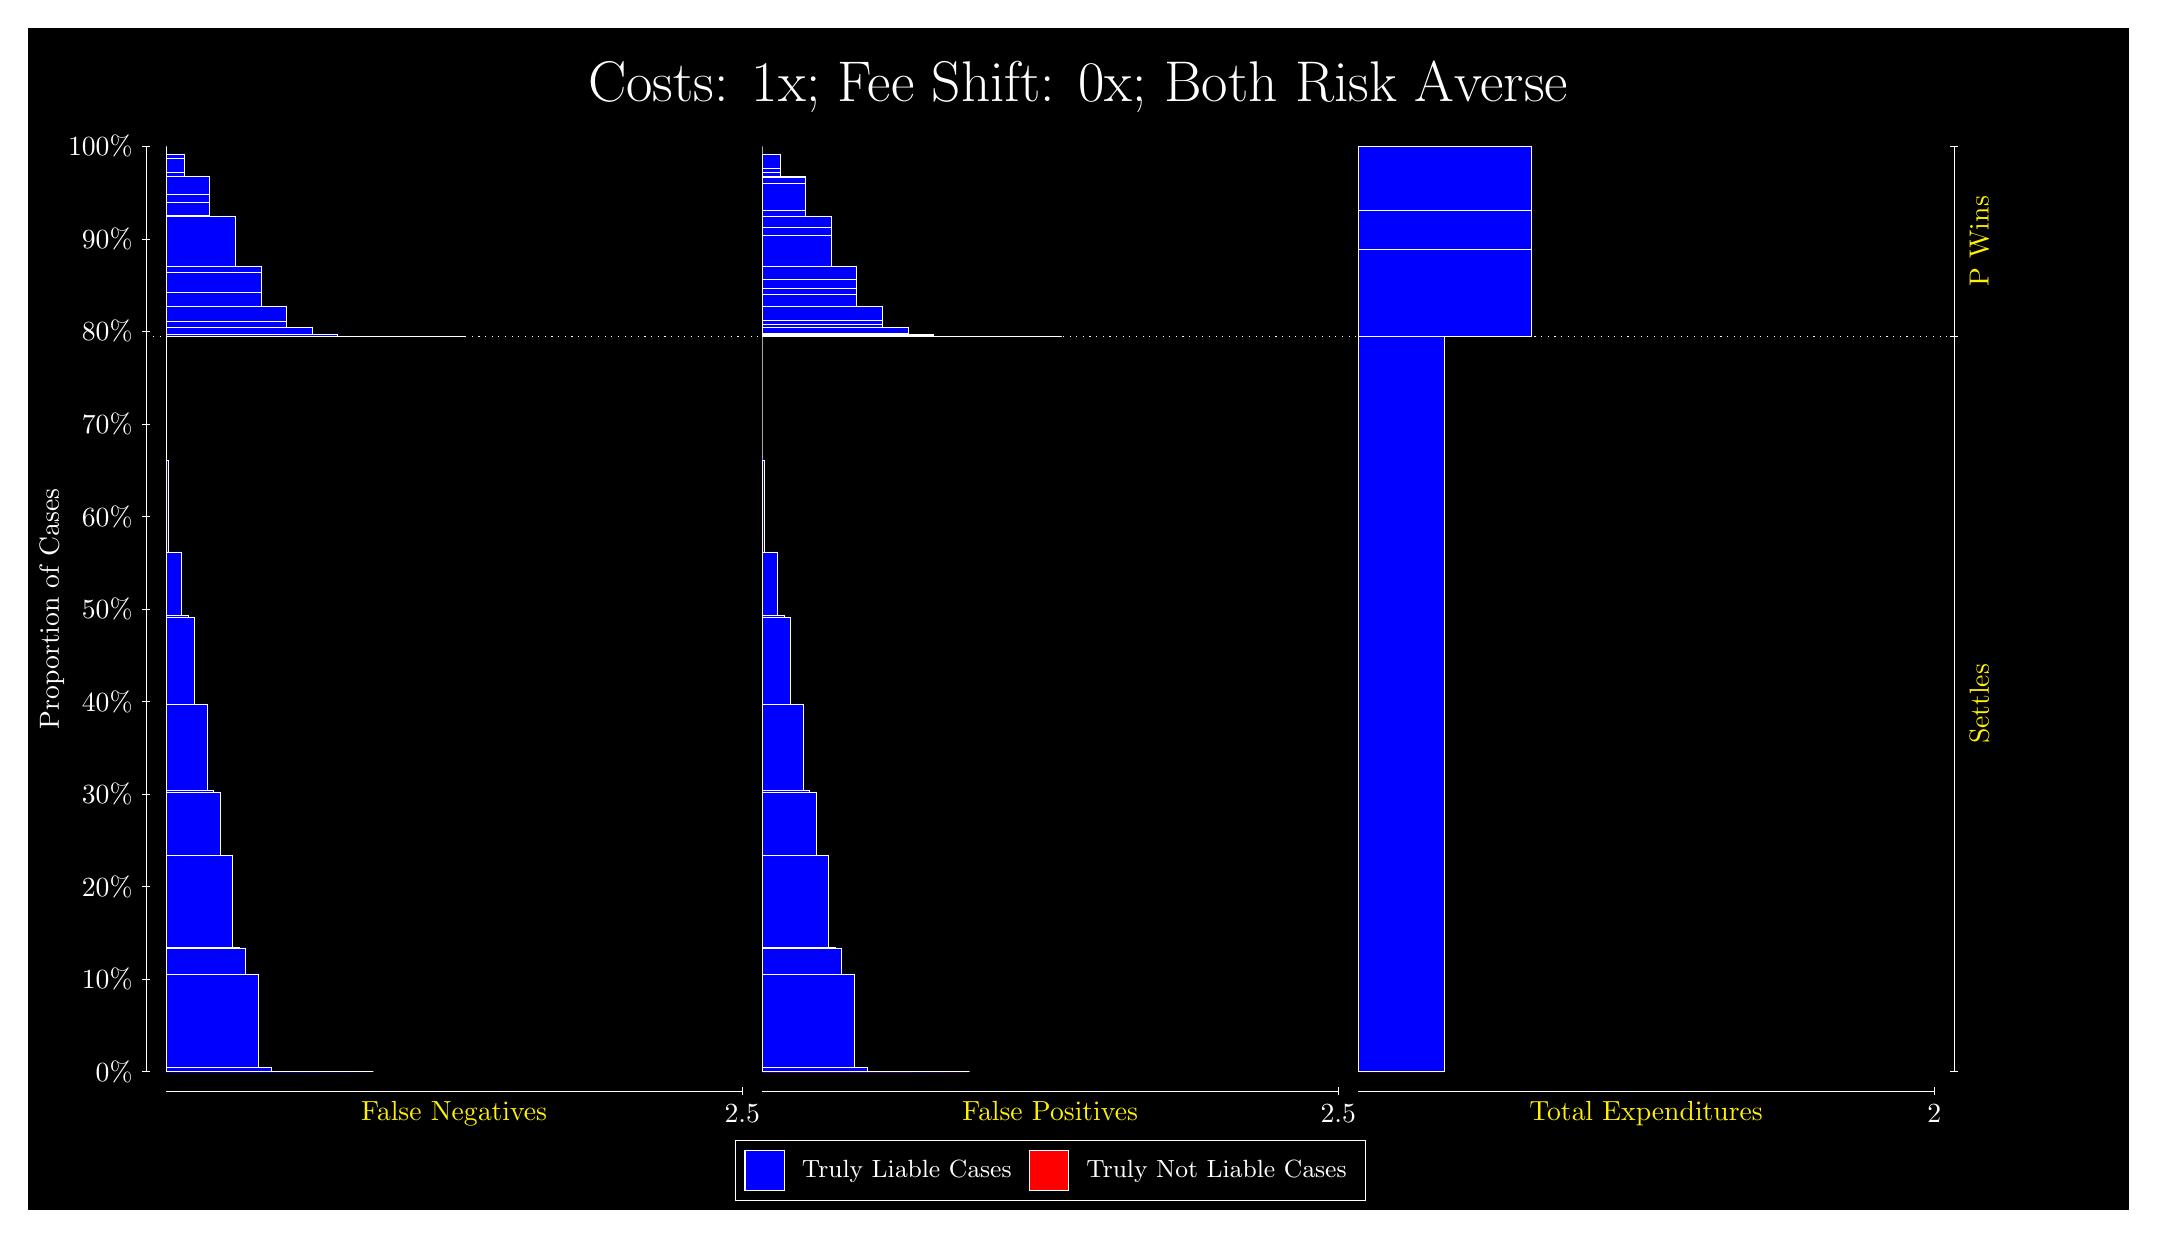
\begin{tikzpicture}
\draw[fill=black] (0,0) rectangle (26.667,15);
\draw[text=white] (0,13.5) rectangle (26.667,15) node[midway] {\huge Costs: 1x; Fee Shift: 0x; Both Risk Averse};
\draw[white, very thin] (1.5,1.75) -- (1.5,13.5);
\node[rotate=90, text=white, anchor=center] at (0.3, 7.625) {Proportion of Cases};
\draw[white, very thin] (1.45,1.75) -- (1.55,1.75);
\node[text=white, anchor=east] at (1.45, 1.75) {0\%};
\draw[white, very thin] (1.45,2.925) -- (1.55,2.925);
\node[text=white, anchor=east] at (1.45, 2.925) {10\%};
\draw[white, very thin] (1.45,4.1) -- (1.55,4.1);
\node[text=white, anchor=east] at (1.45, 4.1) {20\%};
\draw[white, very thin] (1.45,5.275) -- (1.55,5.275);
\node[text=white, anchor=east] at (1.45, 5.275) {30\%};
\draw[white, very thin] (1.45,6.45) -- (1.55,6.45);
\node[text=white, anchor=east] at (1.45, 6.45) {40\%};
\draw[white, very thin] (1.45,7.625) -- (1.55,7.625);
\node[text=white, anchor=east] at (1.45, 7.625) {50\%};
\draw[white, very thin] (1.45,8.8) -- (1.55,8.8);
\node[text=white, anchor=east] at (1.45, 8.8) {60\%};
\draw[white, very thin] (1.45,9.975) -- (1.55,9.975);
\node[text=white, anchor=east] at (1.45, 9.975) {70\%};
\draw[white, very thin] (1.45,11.15) -- (1.55,11.15);
\node[text=white, anchor=east] at (1.45, 11.15) {80\%};
\draw[white, very thin] (1.45,12.325) -- (1.55,12.325);
\node[text=white, anchor=east] at (1.45, 12.325) {90\%};
\draw[white, very thin] (1.45,13.5) -- (1.55,13.5);
\node[text=white, anchor=east] at (1.45, 13.5) {100\%};

\draw[white, very thin] (24.457,1.75) -- (24.457,13.5);
\draw[white, very thin] (24.407,1.75) -- (24.507,1.75);
\node[anchor=west] at (24.407, 1.75) {};
\draw[white, very thin] (24.407,11.089) -- (24.507,11.089);
\node[anchor=west] at (24.407, 11.089) {};
\draw[white, very thin] (24.407,13.5) -- (24.507,13.5);
\node[anchor=west] at (24.407, 13.5) {};

\draw[white, very thin, fill=blue] (1.75,1.75) rectangle (4.3848,1.75);
\draw[white, very thin, fill=blue] (1.75,1.75) rectangle (4.0595,1.75);
\draw[white, very thin, fill=blue] (1.75,1.75) rectangle (3.7342,1.75);
\draw[white, very thin, fill=blue] (1.75,1.75) rectangle (3.6529,1.75);
\draw[white, very thin, fill=blue] (1.75,1.75) rectangle (3.4089,1.7523);
\draw[white, very thin, fill=blue] (1.75,1.7523) rectangle (3.3276,1.7523);
\draw[white, very thin, fill=blue] (1.75,1.7523) rectangle (3.0837,1.8066);
\draw[white, very thin, fill=blue] (1.75,1.8066) rectangle (3.0023,1.8068);
\draw[white, very thin, fill=blue] (1.75,1.8068) rectangle (2.921,2.9814);
\draw[white, very thin, fill=blue] (1.75,2.9814) rectangle (2.7584,3.3198);
\draw[white, very thin, fill=blue] (1.75,3.3198) rectangle (2.6771,3.3248);
\draw[white, very thin, fill=blue] (1.75,3.3248) rectangle (2.5957,4.492);
\draw[white, very thin, fill=blue] (1.75,4.492) rectangle (2.4331,5.2993);
\draw[white, very thin, fill=blue] (1.75,5.2993) rectangle (2.3518,5.3236);
\draw[white, very thin, fill=blue] (1.75,5.3236) rectangle (2.2705,6.4193);
\draw[white, very thin, fill=blue] (1.75,6.4193) rectangle (2.1078,7.5151);
\draw[white, very thin, fill=blue] (1.75,7.5151) rectangle (2.0265,7.5393);
\draw[white, very thin, fill=blue] (1.75,7.5393) rectangle (1.9452,8.3466);
\draw[white, very thin, fill=blue] (1.75,8.3466) rectangle (1.7825,9.5138);
\draw[white, very thin, fill=red] (1.75,9.5138) rectangle (1.75,9.5138);
\draw[white, very thin, fill=blue] (1.75,9.5138) rectangle (1.75,11.089);
\draw[white, very thin, fill=blue] (1.75,11.089) rectangle (5.5558,11.089);
\draw[white, very thin, fill=blue] (1.75,11.089) rectangle (5.2305,11.089);
\draw[white, very thin, fill=blue] (1.75,11.089) rectangle (4.9052,11.089);
\draw[white, very thin, fill=blue] (1.75,11.089) rectangle (4.58,11.089);
\draw[white, very thin, fill=blue] (1.75,11.089) rectangle (4.58,11.089);
\draw[white, very thin, fill=blue] (1.75,11.089) rectangle (4.2547,11.09);
\draw[white, very thin, fill=blue] (1.75,11.09) rectangle (4.2547,11.09);
\draw[white, very thin, fill=blue] (1.75,11.09) rectangle (3.9294,11.107);
\draw[white, very thin, fill=blue] (1.75,11.107) rectangle (3.6041,11.196);
\draw[white, very thin, fill=blue] (1.75,11.196) rectangle (3.2788,11.28);
\draw[white, very thin, fill=blue] (1.75,11.28) rectangle (3.2788,11.464);
\draw[white, very thin, fill=blue] (1.75,11.464) rectangle (2.9535,11.464);
\draw[white, very thin, fill=blue] (1.75,11.464) rectangle (2.9535,11.642);
\draw[white, very thin, fill=blue] (1.75,11.642) rectangle (2.9535,11.898);
\draw[white, very thin, fill=blue] (1.75,11.898) rectangle (2.9535,11.977);
\draw[white, very thin, fill=blue] (1.75,11.977) rectangle (2.6283,11.979);
\draw[white, very thin, fill=blue] (1.75,11.979) rectangle (2.6283,12.612);
\draw[white, very thin, fill=blue] (1.75,12.612) rectangle (2.303,12.629);
\draw[white, very thin, fill=blue] (1.75,12.629) rectangle (2.303,12.789);
\draw[white, very thin, fill=blue] (1.75,12.789) rectangle (2.303,12.888);
\draw[white, very thin, fill=blue] (1.75,12.888) rectangle (2.303,13.124);
\draw[white, very thin, fill=blue] (1.75,13.124) rectangle (1.9777,13.174);
\draw[white, very thin, fill=blue] (1.75,13.174) rectangle (1.9777,13.353);
\draw[white, very thin, fill=blue] (1.75,13.353) rectangle (1.9777,13.393);
\draw[white, very thin, fill=red] (1.75,13.393) rectangle (1.75,13.393);
\draw[white, very thin, fill=blue] (1.75,13.393) rectangle (1.75,13.5);
\draw[white, very thin, fill=red] (9.3189,1.75) rectangle (11.954,1.75);
\draw[white, very thin, fill=blue] (9.3189,1.75) rectangle (11.954,1.75);
\draw[white, very thin, fill=blue] (9.3189,1.75) rectangle (11.628,1.75);
\draw[white, very thin, fill=blue] (9.3189,1.75) rectangle (11.303,1.75);
\draw[white, very thin, fill=red] (9.3189,1.75) rectangle (11.222,1.75);
\draw[white, very thin, fill=blue] (9.3189,1.75) rectangle (11.222,1.75);
\draw[white, very thin, fill=blue] (9.3189,1.75) rectangle (10.978,1.7523);
\draw[white, very thin, fill=blue] (9.3189,1.7523) rectangle (10.896,1.7523);
\draw[white, very thin, fill=blue] (9.3189,1.7523) rectangle (10.653,1.8066);
\draw[white, very thin, fill=blue] (9.3189,1.8066) rectangle (10.571,1.8068);
\draw[white, very thin, fill=red] (9.3189,1.8068) rectangle (10.49,1.8068);
\draw[white, very thin, fill=blue] (9.3189,1.8068) rectangle (10.49,2.9814);
\draw[white, very thin, fill=blue] (9.3189,2.9814) rectangle (10.327,3.3197);
\draw[white, very thin, fill=blue] (9.3189,3.3197) rectangle (10.246,3.3247);
\draw[white, very thin, fill=blue] (9.3189,3.3247) rectangle (10.165,4.4919);
\draw[white, very thin, fill=blue] (9.3189,4.4919) rectangle (10.002,5.2993);
\draw[white, very thin, fill=blue] (9.3189,5.2993) rectangle (9.9206,5.3235);
\draw[white, very thin, fill=blue] (9.3189,5.3235) rectangle (9.8393,6.4192);
\draw[white, very thin, fill=blue] (9.3189,6.4192) rectangle (9.6767,7.515);
\draw[white, very thin, fill=blue] (9.3189,7.515) rectangle (9.5954,7.5392);
\draw[white, very thin, fill=blue] (9.3189,7.5392) rectangle (9.514,8.3466);
\draw[white, very thin, fill=blue] (9.3189,8.3466) rectangle (9.3514,9.5138);
\draw[white, very thin, fill=blue] (9.3189,9.5138) rectangle (9.3189,11.089);
\draw[white, very thin, fill=red] (9.3189,11.089) rectangle (13.125,11.089);
\draw[white, very thin, fill=blue] (9.3189,11.089) rectangle (13.125,11.089);
\draw[white, very thin, fill=red] (9.3189,11.089) rectangle (12.799,11.089);
\draw[white, very thin, fill=blue] (9.3189,11.089) rectangle (12.799,11.089);
\draw[white, very thin, fill=blue] (9.3189,11.089) rectangle (12.474,11.089);
\draw[white, very thin, fill=red] (9.3189,11.089) rectangle (12.474,11.089);
\draw[white, very thin, fill=blue] (9.3189,11.089) rectangle (12.474,11.089);
\draw[white, very thin, fill=blue] (9.3189,11.089) rectangle (12.149,11.089);
\draw[white, very thin, fill=blue] (9.3189,11.089) rectangle (12.149,11.089);
\draw[white, very thin, fill=red] (9.3189,11.089) rectangle (12.149,11.089);
\draw[white, very thin, fill=blue] (9.3189,11.089) rectangle (12.149,11.089);
\draw[white, very thin, fill=red] (9.3189,11.089) rectangle (11.824,11.089);
\draw[white, very thin, fill=blue] (9.3189,11.089) rectangle (11.824,11.09);
\draw[white, very thin, fill=blue] (9.3189,11.09) rectangle (11.824,11.09);
\draw[white, very thin, fill=blue] (9.3189,11.09) rectangle (11.824,11.09);
\draw[white, very thin, fill=red] (9.3189,11.09) rectangle (11.498,11.09);
\draw[white, very thin, fill=blue] (9.3189,11.09) rectangle (11.498,11.106);
\draw[white, very thin, fill=blue] (9.3189,11.106) rectangle (11.498,11.107);
\draw[white, very thin, fill=blue] (9.3189,11.107) rectangle (11.173,11.124);
\draw[white, very thin, fill=red] (9.3189,11.124) rectangle (11.173,11.124);
\draw[white, very thin, fill=blue] (9.3189,11.124) rectangle (11.173,11.196);
\draw[white, very thin, fill=blue] (9.3189,11.196) rectangle (10.848,11.236);
\draw[white, very thin, fill=blue] (9.3189,11.236) rectangle (10.848,11.295);
\draw[white, very thin, fill=red] (9.3189,11.295) rectangle (10.848,11.295);
\draw[white, very thin, fill=blue] (9.3189,11.295) rectangle (10.848,11.464);
\draw[white, very thin, fill=blue] (9.3189,11.464) rectangle (10.522,11.626);
\draw[white, very thin, fill=blue] (9.3189,11.626) rectangle (10.522,11.703);
\draw[white, very thin, fill=red] (9.3189,11.703) rectangle (10.522,11.703);
\draw[white, very thin, fill=blue] (9.3189,11.703) rectangle (10.522,11.815);
\draw[white, very thin, fill=blue] (9.3189,11.815) rectangle (10.522,11.817);
\draw[white, very thin, fill=blue] (9.3189,11.817) rectangle (10.522,11.977);
\draw[white, very thin, fill=blue] (9.3189,11.977) rectangle (10.197,12.376);
\draw[white, very thin, fill=red] (9.3189,12.376) rectangle (10.197,12.376);
\draw[white, very thin, fill=blue] (9.3189,12.376) rectangle (10.197,12.473);
\draw[white, very thin, fill=blue] (9.3189,12.473) rectangle (10.197,12.612);
\draw[white, very thin, fill=blue] (9.3189,12.612) rectangle (9.8718,12.689);
\draw[white, very thin, fill=blue] (9.3189,12.689) rectangle (9.8718,13.03);
\draw[white, very thin, fill=blue] (9.3189,13.03) rectangle (9.8718,13.107);
\draw[white, very thin, fill=blue] (9.3189,13.107) rectangle (9.8718,13.124);
\draw[white, very thin, fill=blue] (9.3189,13.124) rectangle (9.5466,13.174);
\draw[white, very thin, fill=blue] (9.3189,13.174) rectangle (9.5466,13.223);
\draw[white, very thin, fill=blue] (9.3189,13.223) rectangle (9.5466,13.393);
\draw[white, very thin, fill=blue] (9.3189,13.393) rectangle (9.3189,13.5);
\draw[white, very thin, fill=red] (16.888,1.75) rectangle (17.986,1.75);
\draw[white, very thin, fill=blue] (16.888,1.75) rectangle (17.986,11.089);
\draw[white, very thin, fill=red] (16.888,11.089) rectangle (19.083,11.089);
\draw[white, very thin, fill=blue] (16.888,11.089) rectangle (19.083,12.194);
\draw[white, very thin, fill=red] (16.888,12.194) rectangle (19.083,12.194);
\draw[white, very thin, fill=blue] (16.888,12.194) rectangle (19.083,12.694);
\draw[white, very thin, fill=red] (16.888,12.694) rectangle (19.083,12.694);
\draw[white, very thin, fill=blue] (16.888,12.694) rectangle (19.083,13.5);
\draw[white, dotted] (1.5,11.089) -- (24.457,11.089);
\draw[white, very thin] (1.75,1.5) -- (9.0689,1.5);
\node[text=yellow, anchor=north] at (5.4094, 1.5) {False Negatives};
\draw[white, very thin] (9.0689,1.45) -- (9.0689,1.55);
\node[text=white, anchor=north] at (9.0689, 1.45) {2.5};

\draw[white, very thin] (9.3189,1.5) -- (16.638,1.5);
\node[text=yellow, anchor=north] at (12.978, 1.5) {False Positives};
\draw[white, very thin] (16.638,1.45) -- (16.638,1.55);
\node[text=white, anchor=north] at (16.638, 1.45) {2.5};

\draw[white, very thin] (16.888,1.5) -- (24.207,1.5);
\node[text=yellow, anchor=north] at (20.547, 1.5) {Total Expenditures};
\draw[white, very thin] (24.207,1.45) -- (24.207,1.55);
\node[text=white, anchor=north] at (24.207, 1.45) {2};

\node[text=yellow, centered, rotate=90] at (24.777, 6.4193) {Settles};
\node[text=yellow, centered, rotate=90] at (24.777, 12.294) {P Wins};

\draw (12.978300999999998,1.5) node[draw=none] (baseCoordinate) {};
\begin{scope}[align=center]
        \matrix[scale=0.5, draw=white, below=0.5cm of baseCoordinate, nodes={draw}, column sep=0.1cm]{
            \node[rectangle, draw, minimum width=0.5cm, minimum height=0.5cm, fill=blue] {}; &
            \node[draw=none, font=\small, text=white] (B) {Truly Liable Cases}; &
            \node[rectangle, draw, minimum width=0.5cm, minimum height=0.5cm, fill=red] {}; &
            \node[draw=none, font=\small, text=white] (B) {Truly Not Liable Cases}; \\
            };
\end{scope}

\end{tikzpicture}
\end{document}